\documentclass[tikz]{standalone}

\usepackage{amsmath}
\usepackage{lmodern}
\usepackage{pgfplots}
\usepackage{physics}

\usepgfplotslibrary{groupplots}
\pgfplotsset{compat=1.17}

\begin{document}
	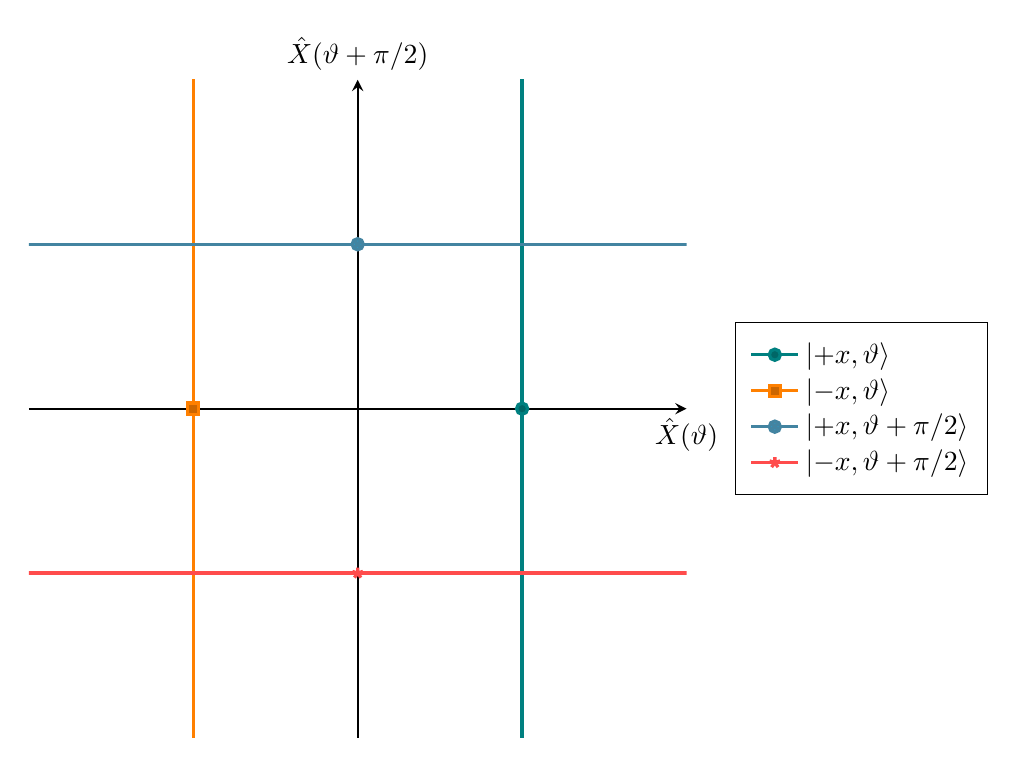
\begin{tikzpicture}
		\begin{axis}[
			width=0.95\linewidth,
			axis lines=center,
			axis equal image,
			xlabel={$\hat{X}(\vartheta)$},
			ylabel={$\hat{X}(\vartheta+\pi/2)$},
			ticks=none,
			xmin=-2,
			xmax=+2,
			ymin=-2,
			ymax=+2,
			axis line style={thick},
			x label style={
				at={(axis description cs:1,0.5)},
				anchor=north,
			},
			y label style={
				at={(axis description cs:0.5,1)},
				anchor=south,
			},
			cycle list name=exotic,
				legend style={
					at={(axis cs: 4,0)},
					anchor=east,
					inner sep=5,
					outer sep=10,
				},
			legend cell align={left},
		]
			\addplot+[very thick] coordinates {(1,-4) (1,0) (1,4)};
			\addlegendentry{$\ket{+x,\vartheta}$};
			\addplot+[very thick] coordinates {(-1,-4) (-1,0) (-1,4)};
			\addlegendentry{$\ket{-x,\vartheta}$};
			\addplot+[very thick] coordinates {(-4,1) (0,1) (4,1)};
			\addlegendentry{$\ket{+x,\vartheta+\pi/2}$};
			\addplot+[very thick] coordinates {(-4,-1) (0,-1) (4,-1)};
			\addlegendentry{$\ket{-x,\vartheta+\pi/2}$};
		\end{axis}
	\end{tikzpicture}
\end{document}